\documentclass{beamer}

\graphicspath{ {./figures/} }
\usepackage{enumitem,xcolor}
\usepackage{tikz}
\usetikzlibrary{mindmap, backgrounds, calc}
\usepackage{subcaption}
\usepackage{natbib}     %% for bibliography
\bibliographystyle{plainnat}

% colored underline, with Beamer overlay support
% usage: \cul{x} or \cul[blue]{x} or \cul<2->{x} or \cul<2->[blue]{x}
\newcommand<>{\cul}[2][red]{%
  % change underline dimentions: https://tex.stackexchange.com/a/167957/25264
  \fontdimen8\textfont3=0.75pt%
  % colored underline: https://tex.stackexchange.com/a/9477/25264
  % transparent underline: https://tex.stackexchange.com/a/45601/25264
  % switch between colored and transparent: http://mirrors.ibiblio.org/CTAN/macros/latex/contrib/beamer/doc/beameruserguide.pdf sections 9.3 and 9.6.1
  \alt#3%
      {\color{#1}\underline{{\color{black}#2}}\color{black}}%
      {\transparent{0.0}\underline{{\transparent{1.0}#2}}\transparent{1.0}}%
}

% so that the captions are numerated
\setbeamertemplate{caption}[numbered]

% when issuing \appendinx in the deocument, these extra slides will not be 
% counted
\renewcommand{\appendixname}{\texorpdfstring{\translate{Appendix}}{Appendix}}

\title{Development of an in-house DORIS processing software}
\author{X. ~Papanikolaou\inst{1} \and V. ~Zacharis\inst{1} 
  \and M. ~Tsichlaki\inst{1} \and S. ~Nahmani\inst{2} 
  \and A. ~Pollet\inst{2} \and M. ~Tsakiri\inst{1} 
  \and J. ~Galanis\inst{1}}
\institute
{
  \inst{1}%
  Dionysos Satellite Observatory\\
  School of Rural, Surveying \& Geoinformatics Engineering\\
  National Technical University of Athens
  \and
  \inst{2}%
  Institut de Physique du Globe de Paris\\
  Université Paris Cité
}
%{\color{blue!20} IDS Workshop, Venice, Italy: October 31 - November 2, 2022 }\date{Nov 01, 2022}
\date{{\color{red!30} IDS Workshop, 
  Venice, Italy: October 31 - November 2, 2022 }}

\begin{document}

\frame{\titlepage}

\begin{frame}{}
\frametitle{Dionysos DORIS Beacon}
Dionysos Satellite Observatory (DSO) has been hosting a DORIS beacon in its 
facilities since 1989. First setup equiped with an \texttt{Alcatel} antenna 
(\ref{fig:dioa}), upgraded in May 2006 to \texttt{Starec} (\ref{fig:diob}).
\begin{figure}
  \centering
  \begin{subfigure}[t]{0.45\textwidth}
    \includegraphics[width=0.7\textwidth]{DIOA}
    \caption{DORIS Beacon DIOA (Alcatel)}
    \label{fig:dioa}
  \end{subfigure}
  \begin{subfigure}[t]{0.45\textwidth}
    \includegraphics[width=1\textwidth]{DIOB_202103}
    \caption{DORIS Beacon DIOB (Starec)}
    \label{fig:diob}
  \end{subfigure}
  \caption{DORIS beacon hosted hosted at DSO facilities}
  \label{fig:dioa-and-diob}
\end{figure}
\end{frame}

\begin{frame}{}
\frametitle{}
Since late 2021, DSO has made the decision to expand its contribution to the 
DORIS community by developing its own, in-house processing software for precise 
orbit determination and positioning using the DORIS system.
\vfill
The software will be designed and build \cul[blue!40]{from scratch}, adopting 
recent developements in DORIS analysis and Satellite Geodesy.
\end{frame}

\begin{frame}{}
\frametitle{Motivation}
\begin{itemize}[label=\textcolor{blue!40}{\textbullet}]
  \item expand out knowledgebase and expertise (research activity \& academic 
    services),
  \item follow and apply state-of-the-art technologies in Satellite Geodesy 
    and expand \& modernize our research activity,
  \item contribute to the DORIS/IDS community, and get invloved ongoing/future 
    projects,
  \item fullfil PhD disertation requirements
\end{itemize}
\end{frame}

\begin{frame}{}
\frametitle{Background}
Up to now, DSO has mainly be involved in precise GNSS positioning, primarily for 
monitoring the crustal dynamics of Greece, a region of complex tectonic \& 
volcanic background.


\begin{itemize}[label=\textcolor{blue!40}{\textbullet}]
  \item since 2015 we have established a monitoring platform using continuous 
    GNSS stations,
  \item daily, routine analysis of an extensive dataset,
  \item contribution to EUREF/EPN Densification (SINEX submission),
  \item time-series analysis (modeling of crustal dynamics)
\end{itemize}

All in all, we have extensive knowledge of GNSS analysis but a limited 
understanding of DORIS technology.
\end{frame}


\begin{frame}{}
\frametitle{Goal}
Our goal is to develop a DORIS analysis software for POD \& positioning.

We follow an incremental approach, intergating one component at a time. As a 
first step, we are targeting:
\begin{itemize}
  \item [\textcolor{blue!40}{\textbullet}] POD-only
  \begin{itemize}
    \item [\textcolor{blue!40}{\textbullet}] Jason-3 satellite
    \item [\textcolor{green!40}{\checkmark}] gradually incorporate more 
      satellites \ldots
  \end{itemize}
  \item [\textcolor{green!40}{\checkmark}] introduce positioning once POD is 
    acceptable
\end{itemize}

Our intention is for the software to be \cul[blue!40]{free of charge }  
and \cul[blue!40]{open-source}, so that the community can benefit as much as 
possible.

Seperate distribution of binaries/scripts and libraries (building is cumbersome).
\end{frame}

\begin{frame}
  \frametitle{Design Considerations (1/2)}
  \begin{itemize}[label=\textcolor{blue!40}{\textbullet}]
    \item Core software development using the \textbf{C++} 
      programming language (exploiting its speed, robustness \& versatility)
    \item Various minor, peripheral parts developed using \textbf{Python}, 
      allowing development speed and ease of use (for developers \& users)
    \item Follow a \textbf{\emph{modular}} design pattern, with different 
      parts developed individually, serving specific needs, thus favoring 
      composability \& reusability
    \item Strive for \textbf{minimum dependencies}; when unavoidable, we 
      only use open-source software
    \item Developed in an ``\textbf{open}'' fashion, using public 
      repositories on \texttt{github}
  \end{itemize}
\end{frame}

\begin{frame}
  \frametitle{Design Considerations (2/2)}
  \begin{itemize}[label=\textcolor{blue!40}{\textbullet}]
    \item RINEX-only processing
    \item We try to follow, as close as possible, the latest IDS 
    recommendations published as 
    ``{\color{red!40}\emph{IDS Recommendations and suggestions for ITRF 2020 reprocessing}}''\footnote{\url{https://ids-doris.org/images/IDS_RecommendationsITRF2020_04.02.2020.pdf}} 
    or design for their easy adoption later on
    \item In general, consulting the extensive documentation on the IDS website 
    ``{\color{red!40}\emph{Documents for the data analysis}}''\footnote{\url{https://ids-doris.org/analysis-coordination/documents-related-to-data-analysis.html}}
    \item Handling of DORIS observations follows the approach outlined in \cite{lemoine-2016} 
      (range-rate)
  \end{itemize}
\end{frame}

\begin{frame}
  \frametitle{Thank you}
  \textbf{Thank you for your attention!}
\end{frame}

\begin{frame}[allowframebreaks]
  \frametitle{References}
    \bibliography{doris}
\end{frame}

\appendix %do not count the following slides for the total number

\begin{frame}
  \frametitle{Not there yet \ldots}
\begin{figure}
  \centering
    \includegraphics[width=0.8\textwidth]{neweop4}
    \caption{Conputed state Vs Sp3 results (Jason3, 02/01/2021)}
    \label{fig:sp3-vs-mine}
\end{figure}
\end{frame}

\begin{frame}
  \begin{figure}
\centering
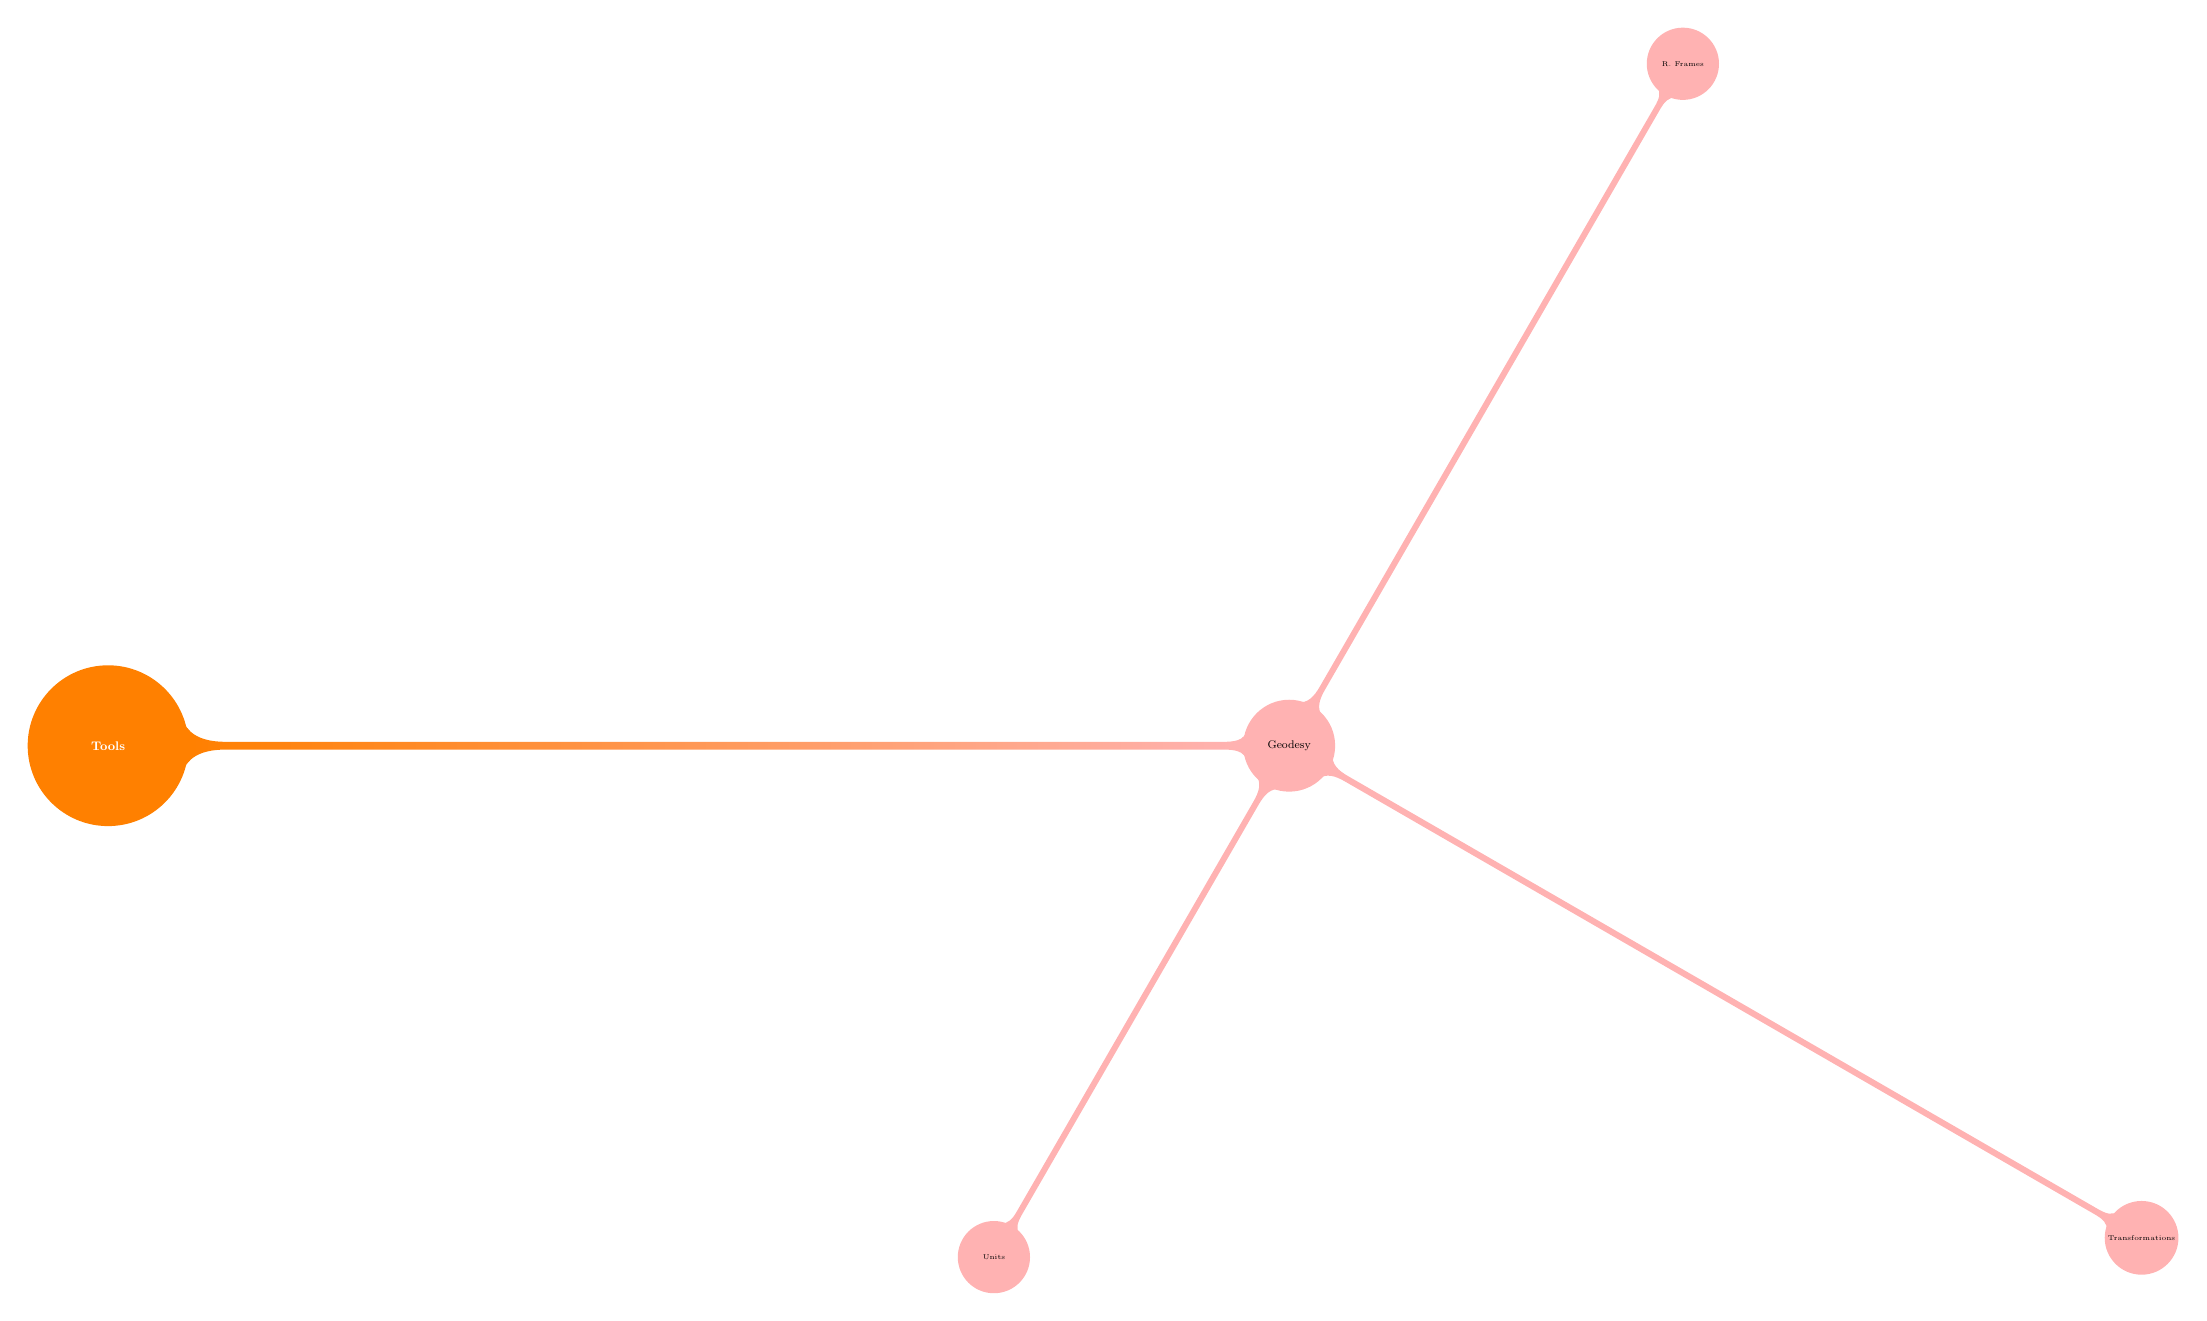
\begin{tikzpicture}[scale=0.5, transform shape,
    mindmap, every node/.style={concept}, grow cyclic, 
    concept color=orange, text=white,
    level 1/.append style={level distance=30cm, sibling angle=70, font=\footnotesize},
    level 2/.append style={level distance=15cm, sibling angle=90}
  ]

  \node{\textbf{\small{Tools}}} [clockwise from=0]
  child [concept color=red!30, text=black, font=\footnotesize, text width=] {
      node {Geodesy} [clockwise from=60]
      child [level distance=20cm, font=\tiny, text width=]{ node {R. Frames}}
      child [level distance=25cm, font=\tiny, text width=]{ node {Transformations}}
      child [font=\tiny, text width=]{ node {Units}}
    };
  %child [concept color=blue!30, text=black, font=\footnotesize, text width=] {
  %    node {Datetimes} [counterclockwise from=250]
  %    child [level distance=20cm, font=\tiny, text width=] { node {Time-Scales}}
  %    child [level distance=20cm, font=\tiny, text width=] { node {Parsing}}
  %  }
  %child [level distance=25cm, concept color=teal, text=white, font=\footnotesize, text width=] {
  %    node {Gravity} [clockwise from=270]
  %    child [font=\tiny, text width=] { node {ICGEM}}
  %    child { node {TVG}}
  %  }
  %child [concept color=red, text=black, font=\footnotesize, text width=] {
  %    node {Math} [counterclockwise from=140]
  %    child { node {EKF}}
  %    child [font=\tiny, text width=] { node {Algebra}}
  %  }
  %child [level distance=23cm, concept color=magenta!60!black, text=white, font=\footnotesize, text width=] {
  %    node {IERS} [counterclockwise from=60]
  %    child [font=\tiny, text width=] { node {Standards}}
  %    child [font=\tiny, text width=] { node {Products}}
  %  };
\end{tikzpicture}
\caption{Software design follows a modular approach, where independent components 
are developed individually; indicative chart.}
\label{fig:software-design}
\end{figure}
\end{frame}
\end{document}